\section{User Acceptance Testing} \label{sec:s4_test}
%%% Intro paragraph

In order to evaluate the usefulness of the crowd condition visualisation from the previous section, we conducted a user acceptance test. This test aims at testing whether the system is ready for use, and is suitable to conclude on the final sprint. In this section we will describe the test and analyse its results.

\subsection{Test Method}

In order to measure the performance of the system, we ask the test subject to analyse a test data scenario, that contains some interesting crowd condition situations. If the system visualises the crowd conditions in a good way, the test subject should be able to understand the crowd conditions.

The test is structured as follows:

\begin{enumerate}
    \item Tutorial scenario
    \item Detailed data set scenario
    \item Evaluation
\end{enumerate}

The test subject should as often as possible navigate the application without the help of the test conductor, in order to observe the intuitiveness of the system. If the test subject is stuck, the test conductor can assist the test subject. Comments and questions are handled on an ad-hoc basis as they naturally arise during the test.

We start the test with a very simple tutorial, consisting of four groups of people with different characteristics. Its purpose is to give the test subject an intuition of how the density, velocity and turbulence overlays behave and the information they can provide. \Cref{fig:tutorial_screens} provides a visual illustration of this. Since the pressure condition would require a more thorough explanation not suitable for this short test, we will not evaluate the pressure overlay in the test.

\begin{figure}[htbp]
\begin{subfigure}[t]{.49\linewidth}
    \centering
    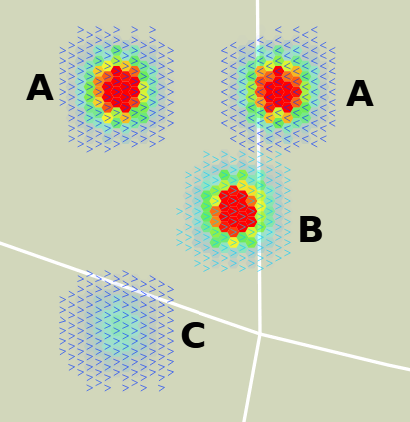
\includegraphics[width=\linewidth]{velocity_density_tutorial.png}
    \caption{Velocity and density - Groups A,B and C are all more dense than group D. Group C moves at a faster rate than the rest.}
\end{subfigure}
\enspace
\begin{subfigure}[t]{.49\linewidth}
    \centering
    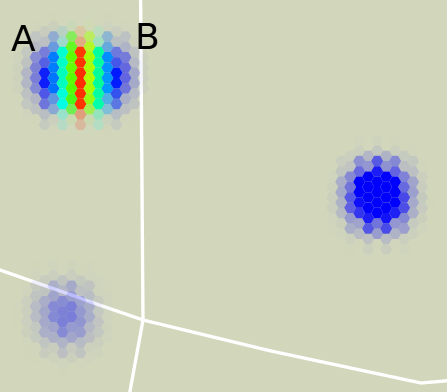
\includegraphics[width=\linewidth]{turbulence_tutorial.png}
    \caption{Turbulence - Groups A and B are \enquote{crashing} which shows up as high turbulence.}
\end{subfigure}
\caption{Screenshots of the tutorial scenario}
\label{fig:tutorial_screens}
\end{figure}

After the tutorial scenario, we will switch to a more detailed data set. The data set is artificially created by us, and resembles a normal day at SmukFest with a variety of interesting situations. \Cref{fig:test_data_screens} illustrates these situations. A large dense crowd is standing in front of a stage, denoted as A. South of the stage, people are moving in a circular walking pattern marked by the dashed lined. This causes a crossroad near the C, where the paths of different groups cross. In the top left corner of the area, near the B, people are moving in opposite directions close to each other, simulating people entering and exiting the festival area.

\begin{figure}[htbp]
\begin{subfigure}[t]{.49\linewidth}
    \centering
    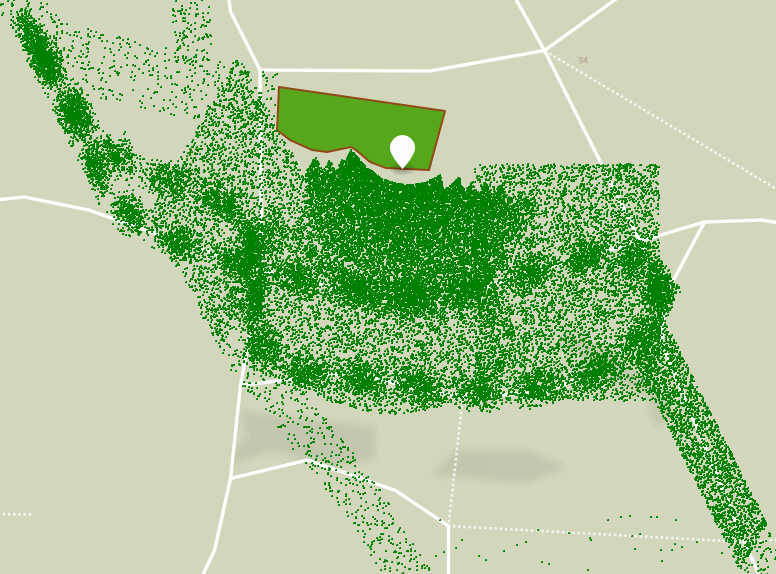
\includegraphics[width=\linewidth]{people_test_data.png}
    \caption{Distribution of people - Each green dot represents a person.}
\end{subfigure}
\enspace
\begin{subfigure}[t]{.49\linewidth}
    \centering
    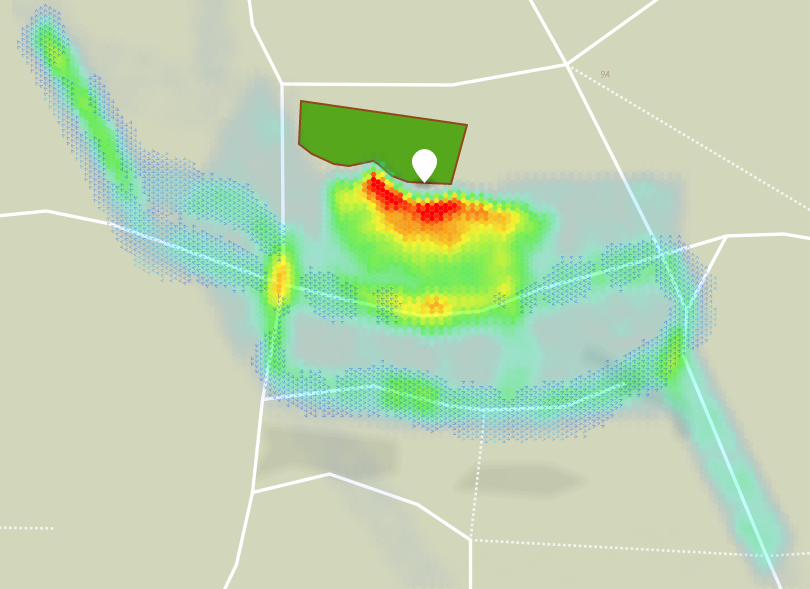
\includegraphics[width=\linewidth]{velocity_density_test_data.png}
    \caption{Velocity and density - The crowd is very dense at center stage, A, and also at a few positions where multiple groups of people meet B, C. Velocity can be seen along the dashed line south of the stage.}
\end{subfigure}
\enspace
\begin{subfigure}[t]{.49\linewidth}
    \centering
    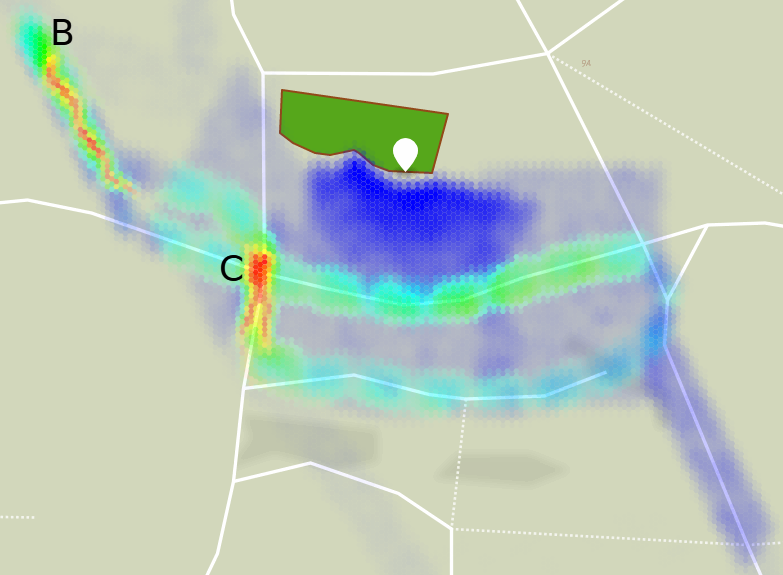
\includegraphics[width=\linewidth]{turbulence_test_data.png}
    \caption{Turbulence - The turbulence is high at two positions; at the crossroads C, and at the festival entrance B. Even though density at center stage is high, the turbulence is low. This indicates that people are standing close to each other, but there is little movement. This would indicate that the high density area in front of the stage is less of a threat.}
\end{subfigure}
\caption{Screenshots of the test data scenario}
\label{fig:test_data_screens}
\end{figure}

The test is successful if the test subject is able to identify all the interesting situations described above. 

Anders Nord of Alarm HS, kindly agreed to participate in this user test. The user test was performed over Skype as in other meetings. Anders was presented with the application which was configured to display the aforementioned predefined crowd scenarios. A summary of the meeting can be seen in \cref{appendix:final_meeting_anders_nord}.

%%% Testing results, high abstraction level
\subsection{Test Results}
Anders immediately noticed, using the density overlay, that the density was high in front of the stage, and at the crossroads where people meet. 

Switching to the velocity overlay, he did not immediately notice the arrows, as they were small. When we hinted that there were arrows, he was able to find the circular movement patterns. Having both the velocity and density overlays enabled at the same time, Anders understood why the density was high at the crossroads; Many groups were heading to the crossroad.

The meaning of the turbulence overlay was not completely clear to Anders as he turned it on, but he quickly noticed that there was no turbulence at the area in front of the stage. His hypothesis was that the crowd was standing still at the area, which we could confirm. He also noticed the high turbulence at the crossroad and at the top left corner.

Overall, Anders was able to find all the interesting situations we had put in the test data, meaning that the visualisations of the system were good. He however expressed that he was not completely confident in his knowledge about what each overlay represents. To overcome this issue, Anders suggested that a user of the system receives some sort of training on the system. 

We can conclude that the test was succesfull, as Anders found all the interesting situations. We need to reconsider the design of the turbulence overlay, as it was not intuitive, and the design of the velocity, as the arrows were difficult to see.


